%	\section{Controller}
	\mypackage{Controller}

Manages interaction with the user and asks the model to execute tasks. 
	\begin{figure}
	\centering
	%\fbox{	
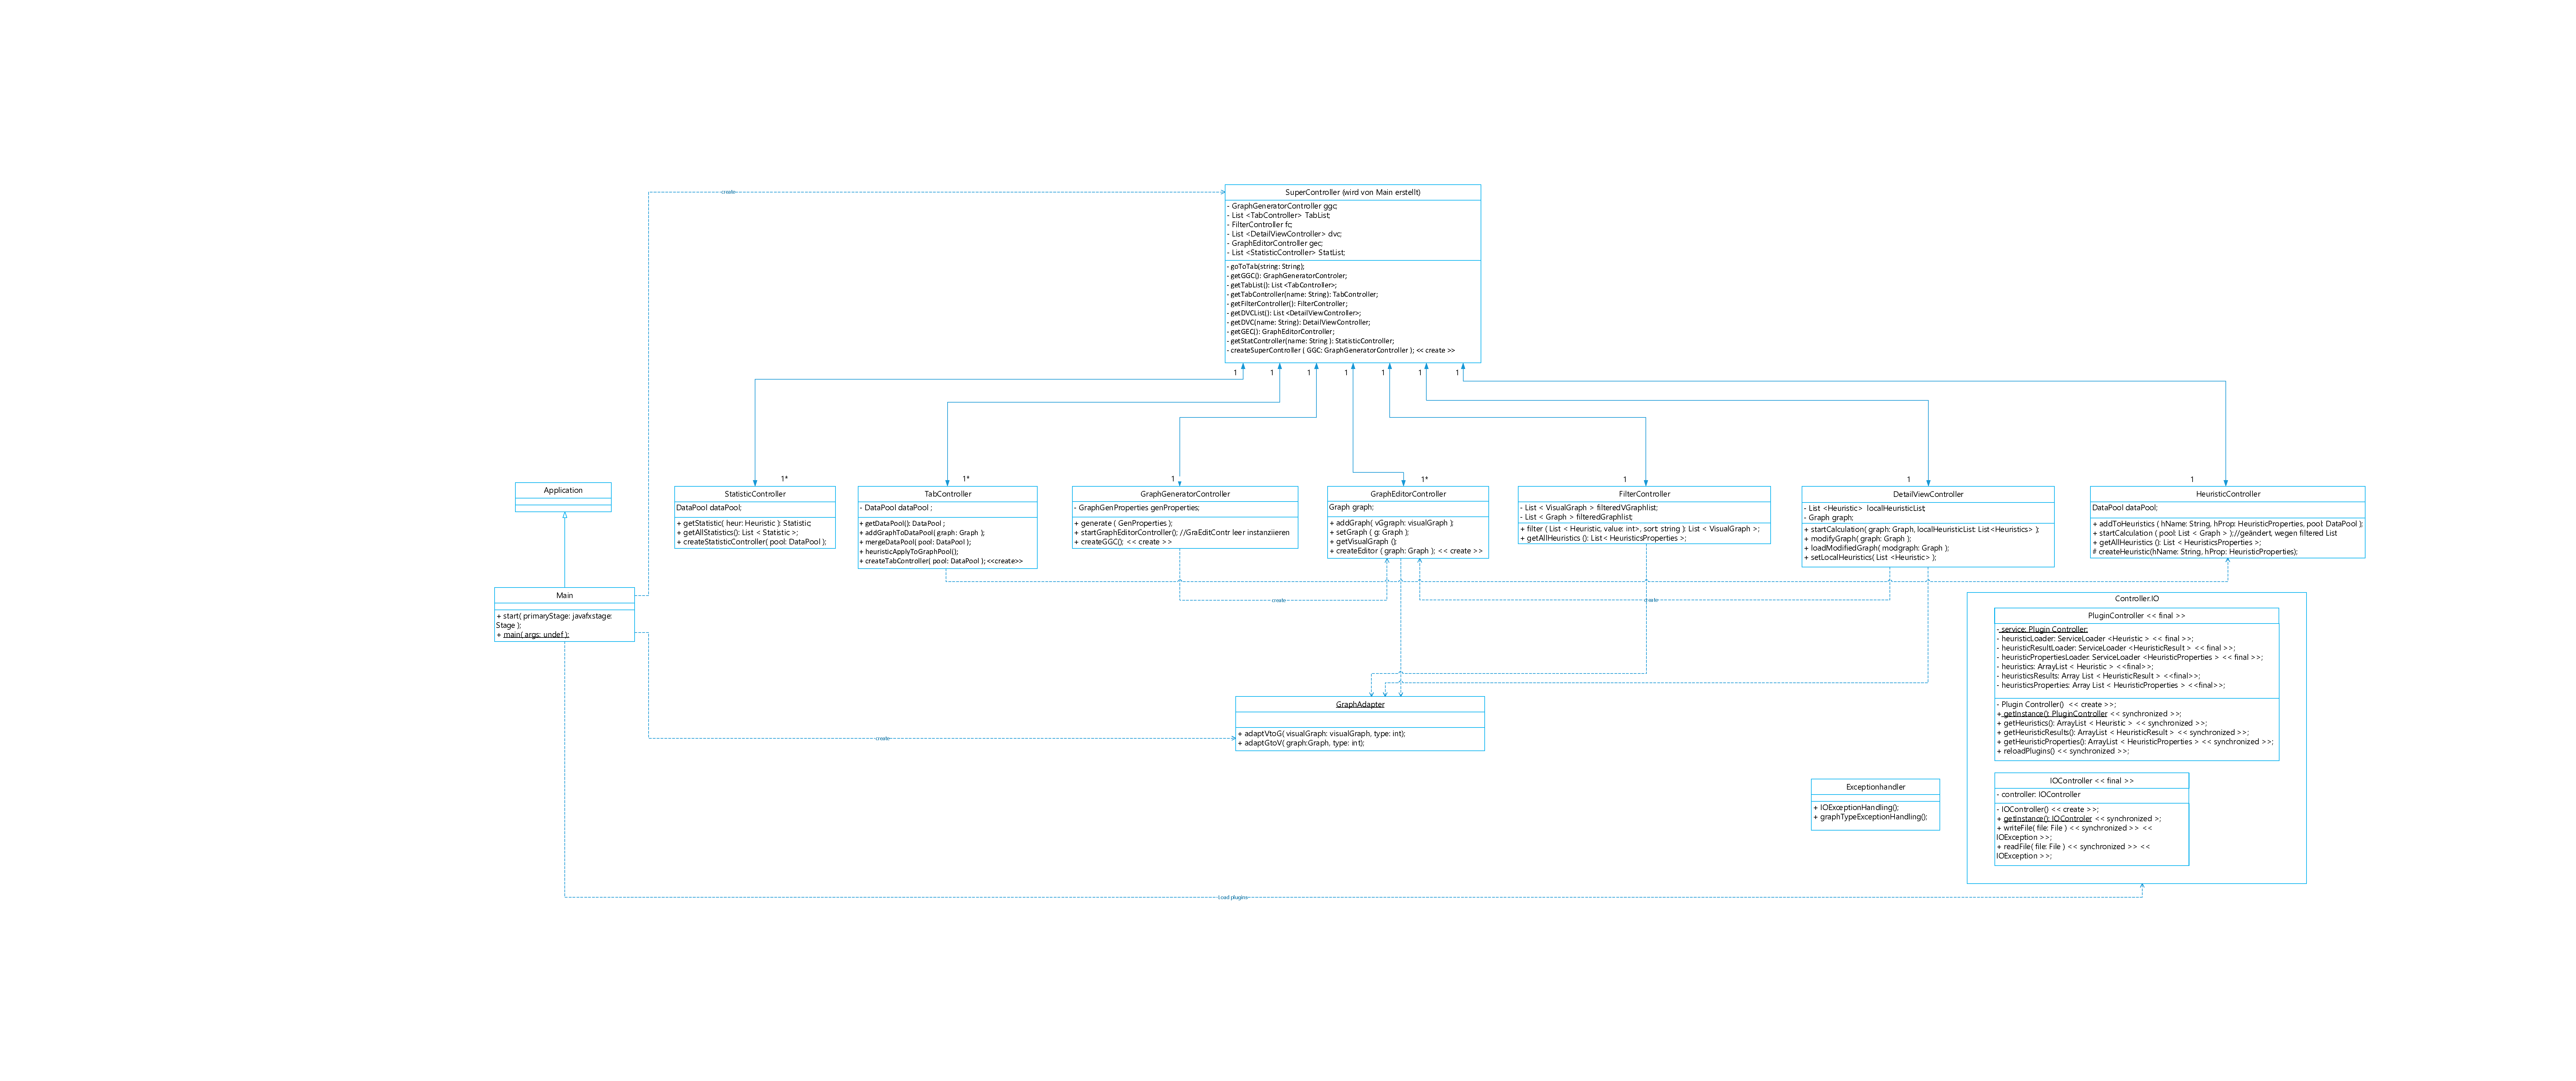
\includegraphics[width=\textwidth]{abbildungen/ControllerOhneMethodenBeschreibung.pdf}
\caption{Controller }
	\label{img:controller}
	\end{figure}

\myclass{SuperController}

\textbf{Description}

The SuperController has one or more instances of theGrapgGeneratorController, List of TabController, GraphEditorController. \newline
\textbf{Documentation}
\begin{enumerate}[+]
	\item{
	\textbf{SuperController} \newline
	Constructor: Creates a SuperController and gives him immedeately a GraphGeneratorController instance.  \newline
	\textbf{@param GGC} The Param GGC is the instance of a GraphGeneratorController. \newline
	}

	\item{
	\textbf{getGGC} \newline
	\textbf{@return} GraphGeneratorController. \newline

	}
	\item{
	\textbf{createGEC} \newline
	Creates a new GraphEditorController with(out) a graph to display.  \newline
	\textbf{@param pool} The DataPool, where the created graph from the user will be added. \newline
	\textbf{@param graphl} The Graphl, that should be modified. \newline
	}
	\item{
	\textbf{getTabList} \newline
	\textbf{@return} List <TabController>. \newline
	}
	\item{
	\textbf{getTabController} \newline
	\textbf{@param name} name is the PreviewTab identifier, with it, the SuperController can \newline
	identify the current TabController, the User is working on. \newline
	\textbf{@return} TabController. \newline
	}
	\item{
	\textbf{getGEC} \newline
	\textbf{@return} GraphEditorController. \newline
	}
	\item{
	\textbf{createTabController} \newline
	Creates a new preview tab, with a graph liast and a heuristics list.  \newline
	\textbf{@param graphList} List of graphs that should be taken to the new tab. \newline
	\textbf{@param heurList} List of heuristics that should be taken to the new tab. \newline
	\textbf{@return} TabController. \newline
	}
	\item{
	\textbf{createTabController} \newline
	Creates a new preview tab with its own DataPool, and calls the GrapgGeneratorController to generate graphs for the DataPool and it will show the graphs in the preview Tab.  \newline
	\textbf{@param GgenPropertiest} The properties, that dictates how the random graph generation generates graphsö. \newline
	\textbf{@return} TabController. \newline
	}
	\item[-]{
		\textbf{PRIVATEMETHODE} etc
	}
\end{enumerate}

\myclass{StatisticController}

\textbf{Description}

Reads the statistics for a heuristic out of the Model and collects them to show it to the View.

\textbf{Documentation}
\begin{enumerate}[+]
	\item{
	\textbf{StatisticController} \newline
	Constructor: Creates a StatisticController and gets himself a DataPool.
	\textbf{@param pool} The DataPool, that the StatisticController belongs to. \newline
}
	\item{
	\textbf{getAllStatistics} \newline
	\textbf{@return} List <Statistic >. \newline
}
	\item{
	\textbf{getStatistic} \newline
	\textbf{@param heur} heur is the Name of the Heuristic, that you want the statistics from. \newline
	\textbf{@return} Statistic. \newline
}
	\item[-]{
		\textbf{PRIVATEMETHODE} etc
	}
\end{enumerate}

\myclass{TabController}

\textbf{Beschreibung}

The Controller of exactly one Preview Tab in the View, that manages the DataPool of this Preview Tab.

\textbf{Dokumentation}
\begin{enumerate}[+]
	\item{
	\textbf{TabController} \newline
	Constructor: Creates a new TabController and connects it with an own DataPool, it also creates an own StatisticController. \newline
	\textbf{@param tabnamel} The name of this TabController. \newline
	\textbf{@param pool} The DataPool, that belongs to the TabController. \newline
}
	\item{
	\textbf{getDVCList} \newline
	\textbf{@return} List <DetailViewController>. \newline
}
	\item{
	\textbf{getDVC} \newline
	\textbf{@param name} The name is the DetailViewController identifier, with it, theTabController can \newline
	identify the current DetailViewController, the User is working on. \newline
	\textbf{@return} DetailViewController. \newline
	}
	\item{
	\textbf{getDataPool} \newline
	\textbf{@return} DataPool \newline
}
	\item{
	\textbf{addGraphToDataPool} \newline
	Adds one Graph to the DataPool, that belongs to the TabController instance. \newline
	\textbf{@param graph} The graph that should be added to the DataPool. \newline
	\textbf{@throws EXCEPTION} if the type of the Graph is not of the same graph type in the DataPool. \newline
}
	\item{
	\textbf{mergeDataPool} \newline
	Merges two DataPools under one of the two TabController. The other TabController with its DataPool remains untouched. \newline
	\textbf{@param pool} The DataPool, that should be copied. \newline
	\textbf{@throws EXCEPTION} if the graph type of both DataPools is not equal.
}
	\item{
	\textbf{getStatisticController} \newline
	\textbf{@return} StatisticController \newline
}
	\item{
	\textbf{getHeuristicController} \newline
	\textbf{@return} HeuristicController \newline
}
	\item{
	\textbf{getFilterController} \newline
	\textbf{@return} FilterController \newline
}
	\item{
	\textbf{heuristicApplyToDataPool} \newline
	Calls the HeuristicController to collor the graphs. \newline
}
	\item{
	\textbf{createHeuristicController} \newline
	Instanciates a HeuristicController and gives him a DataPool.
	\textbf{@param pool} The given DataPool. \newline
}
	\item{
	\textbf{createDetailViewController} \newline
	Instanciates a DetailViewController and gives him a graph to display with all heuristics, that tried to collor it.
	\textbf{@param graphPositionl} The position of the graph in the graph list in the given DataPool. \newline
}
	\item{
	\textbf{createFilterController} \newline
	Instanciates a FilterController and gives him a DataPool.
	\textbf{@param pool} The given DataPool. \newline
}

	\item[-]{
		\textbf{PRIVATEMETHODE} etc
	}
\end{enumerate}
\myclass{GraphGeneratorController}

\textbf{Beschreibung}

The controller for the graph generation communication between the view and the GraphBuilder in the Model.

\textbf{Dokumentation}
\begin{enumerate}[+]
	\item{
	\textbf{GraphGeneratorController} \newline
	Constructor: Creates a GraphGeneratorController. \newline
}
	\item{
	\textbf{generate} \newline
	Commands the GraphBuilder to create random graphs with specific properties. \newline
	\textbf{@param genProperties} The properties, that restrict the randomnes of the GraphBuilder.\newline

}

	\item{
	\textbf{createManuallyGraph} \newline
	Creates an empty GraphEditorController, that adds that manually generated graph from a user.\newline
	It calls the SuperController to start the method createGEC without a DataPool and without a graph.\newline

}
	\item[-]{
		\textbf{PRIVATEMETHODE} etc
	}
\end{enumerate}
\myclass{GraphEditorController}

\textbf{Beschreibung}

Manages the manipulated or created graph by the user and adds it to the right DataPool. \newline

\textbf{Dokumentation}
\begin{enumerate}[+]
	\item{
	\textbf{GraphEditorController} \newline
	Constructor: Creates a GraphEditorController and it will get a DataPool instance. When it was created by the GraphGeneratorController, it will create an GraphEditorController without a graph. \newline
	If it was created by the DetailViesController, it will get a graph to the new instance. \newline
}
	\item{
	\textbf{setGraph} \newline
	Sets the graph of this instance. \newline
	\textbf{@param g} The graph, that belongs to this instance.\newline
}

	\item{
	\textbf{addGraph} \newline
	Adapts the created visualGraph to a Graph and adds the created graph to the DataPool. If there is no DataPool, it will create a new one. \newline
	\textbf{@param vGraph} The created visualGraph. \newline
}
	\item{
	\textbf{getVisualGraph} \newline
	Returns the Graph of this instance as a visualGraph. \newline
}
	\item[-]{
		\textbf{PRIVATEMETHODE} etc
	}
\end{enumerate}
\myclass{FilterController}

\textbf{Beschreibung}

Controlls the filter set by the user and manages the filtered graph pool and the graph pool in the DataPool. \newline

\textbf{Dokumentation}
\begin{enumerate}[+]
	\item{
	\textbf{createFilterController} \newline
	Constructor: Creates a FilterrController and it will get a DataPool instance. \newline
}
	\item{
	\textbf{filter} \newline
	Filters the graph list from the DataPool. \newline
	\textbf{@param List <Heuristic, value: int>} It determines how the list will be filtered. \newline
	\textbf{@param sort} It determines how list will be sorted (decending, ascending ...). \newline
	\textbf{@return} returns List <VisualGraph>, the DataPool remains untouched. \newline
	\textbf{@throws EXCEPTION} if filter and sort are contradictory.\newline
}
	\item{
	\textbf{getAllHeuristics} \newline
	Returns all properties of the used heuristics and the heuristic name is also a heuristic property. \newline
	\textbf{@return} returns List <HeuristicProperties> \newline
}
	\item[-]{
		\textbf{PRIVATEMETHODE} etc
	}
\end{enumerate}
\myclass{DetailViewController}

\textbf{Beschreibung}

Manages the chosen graph and the heuristics that only apply to this graph, the so called local heuristics. \newline

\textbf{Dokumentation}
\begin{enumerate}[+]
	\item{
	\textbf{startCalculation} \newline
	Applies the local Heuristics to the one graph in the DetailView. \newline
	\textbf{@param graph} The graph that get colloerd by the local heuristics. \newline
	\textbf{@param localHeuristicList} The list of local heuristics, that collors the one graph.
}

	\item{
	\textbf{modifyGraph} \newline
	Creates a GraphEditorController instance with the one graph. \newline
	\textbf{@param graph} The graph that should be modified. \newline
}
	\item{
	\textbf{loadModifiedGraph} \newline
	Loads the modified graph into the DataPool and in to the DetailViewController. \newline
	\textbf{@param modgraph} The modified graph. \newline
}
	\item{
	\textbf{addLocalHeuristics} \newline
	Adds the local heuristics chosen by the user to the localHeuristics. \newline
	\textbf{@param List <Heuristic>} The local Heuristics. \newline
}
	\item{
	\textbf{DetailViewController} \newline
	Creates a new Detail View Controller and creates an empty localHeuristicsList. \newline
	\textbf{@param graph} The graph, thatshouldbe loaded in to the DetailViewController. \newline
}
	\item[-]{
		\textbf{PRIVATEMETHODE} etc
	}
\end{enumerate}
\myclass{HeuristicController}

\textbf{Beschreibung}

Manages the chosen graph and the heuristics that only apply to this graph, the so called local heuristics. \newline

\textbf{Dokumentation}
\begin{enumerate}[+]
	\item{
	\textbf{HeuristicController} \newline
	Creates a HeuristicController and gives him a DataPool. \newline
	\textbf{@param pool} The DataPool to give. \newline
}
	\item{
	\textbf{addToHeuristics} \newline
	Applies the chosen heuristics to the heuristic pool in the DataPool. Calls the createHeuristics method. \newline
	\textbf{@param hName } The name of the heuristic. \newline
	\textbf{@param hProp } The properties of the heuristic. \newline
	\textbf{@param pool } The DataPool, where the heuristics belong. \newline
}
	\item{
	\textbf{startCalculation} \newline
	Commands the Heuristics to calculate their results on the graph pool. \newline
	\textbf{@param pool} The graph list.  \newline
	\textbf{@param hpool} The heuristicList of the DataPool, that should calculate the result on the graph list.  \newline
}
	\item{
	\textbf{getAllHeuristics} \newline
	Returns all possible Heuristics. \newline
	\textbf{@return} returns List <HeuristicsProperties>.  \newline
}
	\item[\#]{
	\item{
	\textbf{createHeuristics} \newline
	Get invoked by addToHeuristics and commands the model to create a new heuristic. \newline
	\textbf{@param hName} The heuristic name. \newline
	\textbf{@param hProp} The heuristic properties. \newline
}}
\end{enumerate}